%%%%%%%%%%%%%%%%%%%%%%%%%%%%%%%%%%%%%%%%%%%%%%%%%%%%%%%%%%%%%%%%%%%%%%%%%%%%%%%
% PART II PROJECT DISSERTATION - RECOMMENDER SYSTEMS
%
% Amir H. Hajizamani, ahh29@cam.ac.uk
%
%%%%%%%%%%%%%%%%%%%%%%%%%%%%%%%%%%%%%%%%%%%%%%%%%%%%%%%%%%%%%%%%%%%%%%%%%%%%%%%

\documentclass[a4paper,12pt,twoside,notitlepage]{report}

\author{Amir H. Hajizamani}
\title{CST Part II Individual Project Dissertation - Recommender Systems for 
Social Networks}

\usepackage{verbatim}
\usepackage[T1]{fontenc}
\usepackage{a4wide}
\usepackage{parskip}
\usepackage{hyperref}
\usepackage{url}
\usepackage{amsmath}
%\usepackage{proof}
\usepackage{comment}
\usepackage{engord}

% Conditionals (for draft mode)
\usepackage{ifthen}

% Headers
\usepackage{fancyhdr}

% TOC customisation
\usepackage{tocloft}

% Captions
\usepackage{subfig}
\usepackage{caption}

% Figures
\usepackage{wrapfig}
\usepackage{graphicx}
\usepackage{tikz}
\usetikzlibrary{positioning,mindmap,chains,shapes.misc,arrows,fit}
\usetikzlibrary{decorations.pathmorphing}

% Tables
\usepackage{array}
\usepackage{booktabs}
\usepackage{colortbl}
\usepackage{longtable}

% Palatino font - remove to go back to normal CMR
\usepackage{mathpazo}

% Colour
\usepackage{color}

% Listings (for code snippets ..._
\usepackage{listings}

% Algorithms
\usepackage[boxed]{algorithm}

%\makeindex

\frenchspacing

%%%%%%%%%%%%%%%%%%%%%%%%%%%%%%%%%%%%%%%%%%%%%%%%%%%%%%%%%%%%%%%%%%%%%%%%%%%%%%%
% The BIG DRAFT SWITCH - Set to true to enable draft mode
%
% !!! This will produce extra output that 
%     is not part of the final dissertation !!!

\newboolean{draft}
\setboolean{draft}{false}

%%%%%%%%%%%%%%%%%%%%%%%%%%%%%%%%%%%%%%%%%%%%%%%%%%%%%%%%%%%%%%%%%%%%%%%%%%%%%%%

%%%%%%%%%%%%%%%%%%%%%%%%%%%%%%%%%%%%%%%%%%%%%%%%%%%%%%%%%%%%%%%%%%%%%%%%%%%%%%%
% Definitions

\def\projtitle{Recommender Systems for Social Networks}
\def\authorname{Amir~H.~Hajizamani} 
\def\authoremail{\url{ahh29@cam.ac.uk}}
\def\authorcollege{St.~John's~College}
\def\projsupervisor{Cecilia~Mascolo}

\def\mixurl{\emph{mixcloud.com}}


%%%%%%%%%%%%%%%%%%%%%%%%%%%%%%%%%%%%%%%%%%%%%%%%%%%%%%%%%%%%%%%%%%%%%%%%%%%%%%%
% Custom Environments

\newcommand{\fixme}[1]{\ifdraft{\color{red} {\bf Fixme: \sc #1}}\fi}
\newcommand{\todo}[1]{\ifdraft{\textsf{\color{red} TODO: #1}}\fi}
\newcommand{\remark}[1]{\ifdraft{\textsf{\color{blue} #1}}\fi}

% Some formatting shortcuts
\newcommand{\rulewidth}{300pt}
\newcommand{\halfrule}{
  \begin{center}
    {\rule{\rulewidth}{0.5pt}}
  \end{center}}

%% Colours
\definecolor{darkgreen}{rgb}{0,0.3137,0.196}
\definecolor{commentgreen}{rgb}{0.247,0.5,0.3725}
\definecolor{darkpurple}{rgb}{0.5,0,0.33}

%% Some shortcuts for maths stuff
\providecommand{\Fm}{\mathtt{F}}
\providecommand{\Pm}{\mathtt{P}}
\providecommand{\Tp}{\textsuperscript{\textsf{T}}}
\providecommand{\xsub}[1]{\mathbf{x}_{#1}}
\providecommand{\X}{\mathbf{X}}
\providecommand{\Pmc}[2]{\mathbf{p}_{#1}^{#2\textsf{T}}}

%% TikZ command for line annotations
% Draw line annotation
% Input:
%   #1 Line offset (optional)
%   #2 Line angle
%   #3 Line length
%   #4 Line label
%   #5 Line colour
% Example:
%   \lineann[1]{30}{2}{$L_1$}
\newcommand{\lineann}[5][0.5]{%
    \begin{scope}[rotate=#2, #5,inner sep=2pt]
        \draw[dashed, #5!40] (0,0) -- +(0,#1)
            node [coordinate, near end] (a) {};
        \draw[dashed, #5!40] (#3,0) -- +(0,#1)
            node [coordinate, near end] (b) {};
        \draw[|<->|] (a) -- node[fill=white] {#4} (b);
    \end{scope}
}

%%%%%%%%%%%%%%%%%%%%%%%%%%%%%%%%%%%%%%%%%%%%%%%%%%%%%%%%%%%%%%%%%%%%%%%%%%%%%%%

\setcounter{page}{1}    % initialise page counter

% pre-TOC page formatting
\pagenumbering{roman}
\pagestyle{plain}

\setcounter{secnumdepth}{2}
\setcounter{tocdepth}{3}

\setlength{\parindent}{0pt}
\setlength{\parskip}{6pt}
\linespread{1.2}

\lstset{    basicstyle=\footnotesize\ttfamily, 
            keywordstyle=\color{purple},
            commentstyle=\color{commentgreen}\textit,
            captionpos=b
        }

\begin{document}

%%%%%%%%%%%%%%%%%%%%%%%%%%%%%%%%%%%%%%%%%%%%%%%%%%%%%%%%%%%%%%%%%%%%%%%%%%%%%%%
% Title Page

\thispagestyle{empty} 

\begin{flushright}
\authorname
\end{flushright}
\bigskip % have this so that vfill works to centre the title vertically

\vfill

\begin{center}
 \medskip
 {\Large\bf \projtitle}

 \vspace*{1cm}

 {\large Computer Science Tripos Part II}

 \bigskip

 {\large \authorcollege}

 \bigskip

 {\large \today}
\end{center}

\vfill

\cleardoublepage


%%%%%%%%%%%%%%%%%%%%%%%%%%%%%%%%%%%%%%%%%%%%%%%%%%%%%%%%%%%%%%%%%%%%%%%%%%%%%%%
% Proforma
\section*{Proforma}

\begin{tabular}{ll}
Name:               & \bf \authorname \\
College:            & \bf \authorcollege \\
Project Title:      & \bf \projtitle \\
Examination:        & \bf Computer Science Tripos, Part II, June 2011 \\
Word Count:         & \bf \todo{~4000 words atm} \\
Project Originator: & \bf \authorname \\
Supervisor:         & \bf \projsupervisor \\
\end{tabular}

%\footnotetext[1]{This word count was computed
%by {\tt detex diss.tex | tr -cd '0-9A-Za-z $\tt\backslash$n' | wc -w}}

\subsection*{Original Aims of the Project}

To build a system that would recommend new social links to users of a social
network in order to increase the connectivity of its social graph. These
recommendations would be based on the current state of the graph and their
quality would depend on whether the recommended links actually occur in a
future state of the graph. From the outset, the dataset to be used for the
project was that of the online audio-sharing community \mixurl.

\subsection*{Work Completed}
I modelled the Mixcloud dataset's entities and wrote an abstraction layer for
the Mixcloud API. I used this in a crawler program that downloaded and stored
the data from \mixurl.

The recommender system I wrote achieves the above aims by modelling the
recommendation process as an edge prediction problem: given a social graph,
it tries to predict what edges are most likely to form in the future between
unconnected nodes and assigns a confidence value to the predictions. This is
done by calculating similarity values between nodes and choosing the most
similar unconnected nodes as predictions.

\subsection*{Special Difficulties}

None.

\newpage

%%%%%%%%%%%%%%%%%%%%%%%%%%%%%%%%%%%%%%%%%%%%%%%%%%%%%%%%%%%%%%%%%%%%%%%%%%%%%%%
% Declaration of Originality
\section*{Declaration}

I, \authorname~of \authorcollege, being a candidate for Part II of the Computer
Science Tripos, hereby declare that this dissertation and the work described in
it are my own work, unaided except as may be specified below, and that
the dissertation does not contain material that has already been used to any
substantial extent for a comparable purpose.

\bigskip
\bigskip
\bigskip
\leftline{Signed}

\medskip
\leftline{Date}


\clearpage

%%%%%%%%%%%%%%%%%%%%%%%%%%%%%%%%%%%%%%%%%%%%%%%%%%%%%%%%%%%%%%%%%%%%%%%%%%%%%%%
% Acknowledgements

\section*{Acknowledgements}

If this dissertation had turned out as I had hoped, I would be thanking those
few special individuals who have encouraged and supported me over the last
three years. But as it is, I have let them down, and my gratitude shall remain
unexpressed for now.

%\begin{itemize}
% \item {\bf Liam~McNamara}, for all the insightful advice along the way and
%generally being an awesome guy.
% \item {\bf Helen~Ennos}, for all her encouragement and support. Without her,
%my
%time at Cambridge would have been a very different experience. 
%\end{itemize}

\cleardoublepage

%%%%%%%%%%%%%%%%%%%%%%%%%%%%%%%%%%%%%%%%%%%%%%%%%%%%%%%%%%%%%%%%%%%%%%%%%%%%%%%
% Table of Contents
\tableofcontents
\clearpage

\clearpage
\listoffigures

\clearpage
\listoftables

\clearpage
\lstlistoflistings

\cleardoublepage


%%%%%%%%%%%%%%%%%%%%%%%%%%%%%%%%%%%%%%%%%%%%%%%%%%%%%%%%%%%%%%%%%%%%%%%%%%%%%%%

% Switch to arabic page numbers after TOC
\setcounter{page}{1}
\setcounter{chapter}{0}
\pagenumbering{arabic}
\pagestyle{headings}


%%%%%%%%%%%%%%%%%%%%%%%%%%%%%%%%%%%%%%%%%%%%%%%%%%%%%%%%%%%%%%%%%%%%%%%%%%%%%%%
% Introduction
\chapter{Introduction}

% - Mention fulfillment early
% - Principal Motivation
% - Other CS work

In this chapter I will explain my motivations for investigating recommender
systems in general and the specific focus points of my project as
presented in this dissertation using data from \mixurl.

\halfrule

\section{Motivation}

The basic concept that underpins recommender systems is that the value of data
about an individual person or piece of content is increased by knowledge of its
relation to other such entities. This is true for the user of a system, whose
experience is enriched with this metadata and is thus incentivised to keep
using, it and the service provider, whose cultural impact and financial success
will depend the growth and interactions of its users with the service.

There are now a growing number of available social networking services that
individuals can choose to invest time and effort into. We take this investment
by the user to consist of: providing personal information, creating and sharing
content, making social connections with other users, and interacting with other
users and content. One way of providing an incentive to do this is by making it
easier for users to make \emph{discoveries} -- to find other individuals or
items of interest (real-world friends, content that compliments the user's
favourites). That is, make recommendations to users and keep them interested in
exploring what the social network has to offer. Recommender systems aim
to solve the problem of \emph{information overload} in areas where the users of
a service struggle to make good choices on what content to consume or what
social activities to take part in, simply because the options are overwhelming.

If we treat the users of a social network as a community, it is clear that such
a community will need the investment mentioned above from its users to reach
some critical mass -- the point at which it is valuable for others to join 
or contribute to the network\footnote{Best described by Beckstrom's Law - The
value of a network equals the net value added to each user's transactions
conducted through that network, summed over all users.} because the majority of
their friends have, or so much of the content they consume is accessible via the
service. This will continually increase the richness and quality of the service
the community receives (assuming the service provider keeps up and adapts to
changes!) and increase the lifetime and utility of the service for its users,
too. Of course, here we are concerned with social networks that aim to reach the
mainstream and are not inherently limited to a select number of users. For
instance, a social network for the community of world experts on network
congestion analysis is bound to hit its maximum membership limit very quickly
and not be much more useful to its users than email or more traditional
communication methods.

From a commercial perspective of a service provider, having users remain active
on the network and incentivise others to do so, too, is paramount. It is
well-understood that social network service providers are not expected to be
profitable\footnote{The 
risks underlying the business of social networks -- 
\url{http://www.makeuseof.com/tag/how-do-social-networks-make-money-case-wondering/}} 
until they reach an ``audience of scale'' to enable the adoption of a sensible 
monetisation model. For instance, Facebook only became profitable in 2009\footnote{
\url{http://www.pcpro.co.uk/news/351646/facebook-eyes-profit-as-it-hits-300-million-members}} 
after reaching 300 million users. This means that the investors who enable such 
ventures at the start need to be convinced that the service has the potential 
to reach popularity and therefore provide a return on investment. Of the many 
strategies that can be used to maintain the growth of a social network, 
implementing a good friend recommender system is standard practice. It should be
noted that recommendations are difficult, if not infeasible, to make at the
very beginning of a network's lifetime due to the \emph{cold start} problem,
that is, when there is insufficient data to base recommendations on. Therefore,
the focus of this project is on stages of a network's lifetime when it is
nearing maturity and this issue hasbeen overcome.

\subsection{Wider Context}

The Web is rife with successful recommender systems, with companies such as 
\emph{Amazon, Netflix\footnote{In 2006 Netflix challenged programmers to 
improve their movie recommendation engine by 10\%.}} and \emph{Pandora} 
(radio service backed by \emph{The Music Genome Project}\footnote{The MGP 
uses the``genealogy'' of music to link songs and artists -- 
\url{http://www.pandora.com}}) investing a lot of time and money in improving 
their algorithms and data quality to better recommend items of interest to 
their users. On the other hand, more directly community-driven websites such as 
\emph{del.icio.us} and \emph{flickr} have harnessed the collective 
intelligence of their users and their tagging of their content with keywords. 
Collaborative tagging leads to an organic categorisation and annotation of data 
which has been termed \emph{folksonomy}\footnote{A portmanteau of 
\emph{folk} and \emph{taxonomy} -- 
\url{http://www.vanderwal.net/folksonomy.html}}. In a sufficiently large and 
active community, the folksonomy that can be extracted becomes a good source of 
input for the algorithms in a recommender system. 

With the accelerating growth of social networks such as Twitter and Facebook, 
the value of social recommendations which aim to increase the connections 
between individuals is more important that it used to be: the items of 
interests are now other users not products on sale (though from an advertising 
revenue perspective the difference is blurred). Recommender systems are nearing 
maturity and will soon be, if they are not already, commodity technologies as 
the ``social connections layer'' of virtual communities is completed\footnote{
The ``game layer'' is the next stage in building virtual communities, the 
founder of SCVNGR argues -- \url{
http://www.ted.com/talks/seth_priebatsch_the_game_layer_on_top_of_the_world.html
}}. 
This means that an analysis of such systems is essential to the understanding 
of social networking and the Web as it experiences a paradigm shift from a 
\emph{search} platform (e.g. Google) to a \emph{discovery} platform.


\section{The \mixurl\ Dataset}

\mixurl\ are a successful audio content distribution website, aiming to be the
``YouTube of Radio''. They provide a platform for user-generated audio content,
ranging from podcasts to DJ mixes, to be easily accessed by anyone. They have
been operating for nearly two years and have in the order of 100,000 users and a
similar number of so-called ``Cloudcasts'' (uploaded audio content). They
provide their niche community of users with social networking features such as
Twitter-style following, Facebook-style activity updates, favouriting of
Cloudcasts and commenting, and a record of listening history. The user-uploaded
Cloudcasts are also heavily annotated with tags, categories, text descriptions
and other metadata. This wealth of metadata about Mixcloud's users and content
is available via their public API\footnote{\url{http://api.mixcloud.com}} and I
gathered the data I need from it.

\subsection{Focus on Social Recommendations}
At the time of writing, \mixurl\ implements some simple mechanisms for 
\emph{item recommendations} and \emph{personalised recommendations}: 
respectively, recommending Cloudcasts similar to the one being viewed/played,
and recommending Cloudcasts related to the user's personal listening history. 

My approach is to provide \emph{social recommendations}: suggesting \emph{other
users} whom the current user may be interested in following or listening to. My
reason for this is that the social aspect of the \mixurl\ community is more
similar to that of Twitter, where people connect with users who produce good
content as well as real life friends, than that of Facebook where social links
are more often initiated physically, or in the traditional sense of ``social''.

Given the motivations for building recommender systems described above, I
understand that the Mixcloud team have prioritised the implementation of 
the recommendations centred around content because their main
focus has been on building up the library of content on their network and
promoting themselves as content distributors. However, the social networking
layer on top of their distribution layer is the next natural focus. 

\subsection{The Temporal Dimension}

As I am collecting my own data firsthand, I can look at the performance of my
recommendations over snapshots of the dataset at different points in time. This
approach could be very interesting because changes to the dataset over time
could be taken to be the ground truths that my recommender system would be
trying to replicate.


\subsection{Comparison with other Available Datasets}

The most widely used datasets in discussions on recommender systems are the 
MovieLens, EachMovie, Book-Crossing and Jester Jokes datasets\footnote{
All of these datasets are available via \url{http://www.grouplens.org/node/12}} 
which contain items and user ratings on their respective titular item types. 
Though the quality of these datasets is proven, they have limitations for my 
intended project goals. In particular, there is no social connectivity data 
between users in these datasets and the links between entities are limited to 
ratings by users on some items. With the Mixcloud dataset I am able to explore 
the social graph of the users. Furthermore, the Mixcloud dataset provides much 
richer metadata about its entities, as described above, than any of these 
traditional datasets which give only enough data to make item
recommendations. The Mixcloud dataset has scope for more interesting analysis.

%%%%%%%%%%%%%%%%%%%%%%%%%%%%%%%%%%%%%%%%%%%%%%%%%%%%%%%%%%%%%%%%%%%%%%%%%%%%%%%
% Preparation 
\chapter{Preparation}

This chapter describes how I refined the ideas presented in my project proposal
before writing any code, and the working environments and best practices I
adopted to minimise problems during the implementation stage.

\halfrule

\section{The Anatomy of the \mixurl\ Dataset}
\label{sec:mix-anatomy}

It is important to understand the nature of the dataset that I use in this
project. What follows is some semantics of how the data is structured, accessed
and presented. 

The general notion underlying \mixurl\ is that producers of audio
content (so-called \emph{Cloudcasts}) and their listeners are users of the
website, and any user can upload content with rich metadata including artist and
track information. The users can then listen to and favourite content, and
furthermore, they can follow other users in whom they are interested, either
socially or because of their content.

All the above data can be obtained from Mixcloud via their Application
Programming Interfact (API) and I break this down in the following subsections.

\begin{figure}
 \centering
 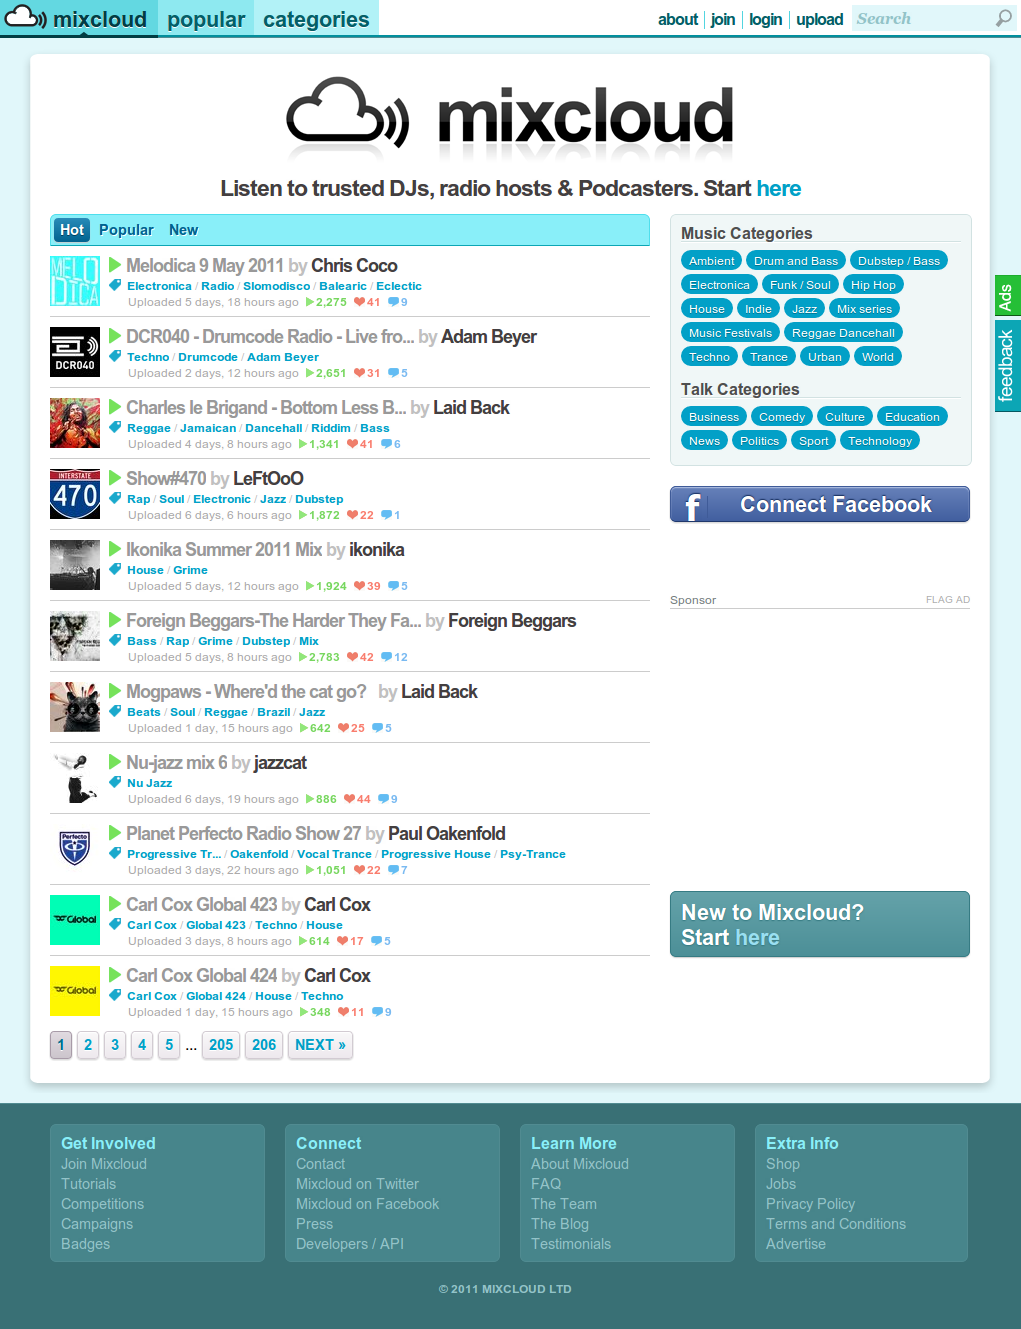
\includegraphics[width=\textwidth]{./images/mixcloud-home.png}
 % mixcloud-home.png: 1021x1329 pixel, 72dpi, 36.02x46.88 cm, bb=0 0 1021 1329
 \caption{\mixurl\ Homepage}
 \label{fig:mix-home}
\end{figure}

\begin{figure}
 \centering
 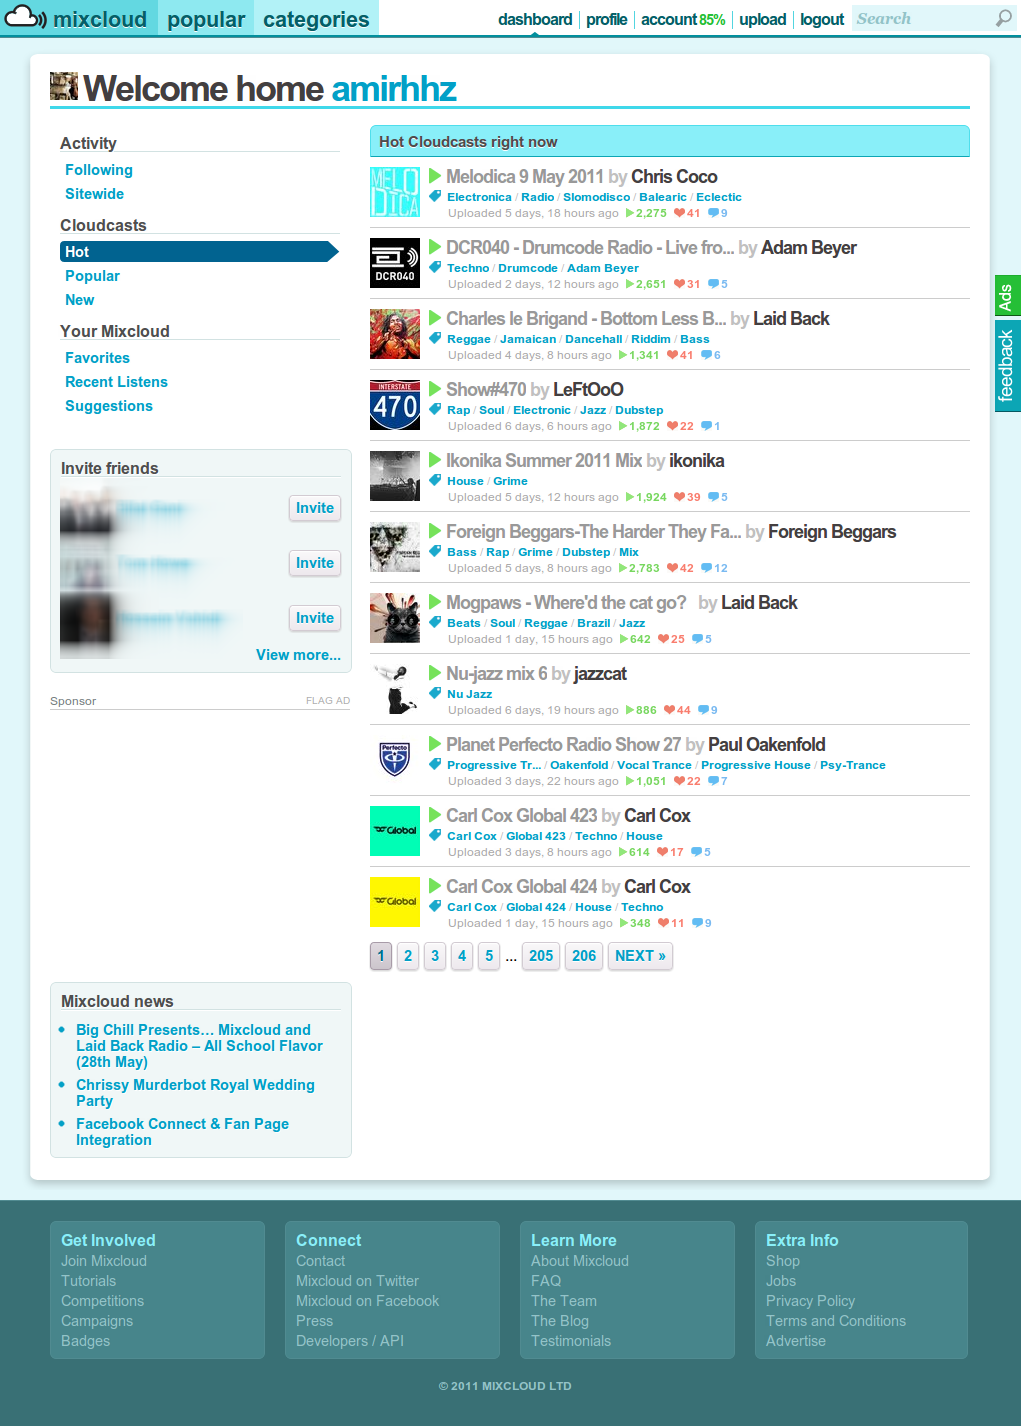
\includegraphics[width=\textwidth]{./images/mixcloud-dashb.png}
 % mixcloud-home.png: 1021x1329 pixel, 72dpi, 36.02x46.88 cm, bb=0 0 1021 1329
 \caption{\mixurl\ Dashboard for logged-in user}
 \label{fig:mix-dash}
\end{figure}

\subsection{The Mixcloud API: A RESTful Exchange of JSON}

The Mixcloud API, accessible via HTTP requests on \url{http://api.mixcloud.com},
allows for the retrieval of data about the various entities and relationship
described above, such as users and cloudcasts. The API responds to HTTP methods
with a JSON\footnote{JavaScript Object Notation}-formatted representation of
the data (see subsection \ref{subsec:nonrel} for more details) for the resource
specified by the URL path. So, for instance, a HTTP
GET request sent to \url{http://api.mixcloud.com/amirhhz} will respond with a
body containing my user information as follows:

\begin{lstlisting}[language=Java,caption=Sample response from the Mixcloud API,
label=lst:api-sample]
{
    "username": "amirhhz", 
    "city": "", 
    "cloudcast_count": 0, 
    "following_count": 11, 
    "url": "http://www.mixcloud.com/amirhhz/", 
    "pictures": {
        "small": /* URL OMMITTED */, 
        "large": /* URL OMMITTED */, 
        "medium": /* URL OMMITTED */, 
    }, 
    "listen_count": 20, 
    "updated_time": "2011-04-13T18:36:57Z", 
    "created_time": "2009-09-07T19:10:17Z", 
    "biog": "", 
    "key": "/amirhhz/", 
    "country": "United Kingdom", 
    "follower_count": 28, 
    "favorite_count": 4, 
    "name": "amirhhz"
} 
\end{lstlisting}

The Mixcloud API adheres to the Representational State Transfer (REST)
style of software architecture, a simple idiom: clients send requests for the
state of a resource to servers and receive an appropriate response containing a
representation of the resource's state at the time. HTTP follows this simple
idiom with its simple methods (e.g. GET, POST, DELETE) and RESTful API's such as
Mixcloud's simply specialise this mechanism to suit their needs of Creating,
Reading, Updating, and Deleting (CRUD) resources on servers as requested by
clients.

\subsection{Base Resources}
In the context of the Mixcloud API, I shall refer to resources in Table 
\ref{tab:base-resources} as \emph{base
resources}.


\begin{table}[h]
  \begin{center}
  \begin{tabular}{r >{\ttfamily}l<{\normalfont}}
Base Resource 	& \textnormal{API path scheme} \\
\hline
User 		& /<user>/ \\
Cloudcast	& /<user>/<cloudcast>/ \\
Tag 		& /tag/<tag>/ \\
Category 	& /categories>/<category>/ \\
Artist 		& /artist/<artist>/ \\
Track		& /track/<artist>/<trackname>/ \\

  \end{tabular}
   
  \end{center}
\caption{Mixcloud API Base Resources and their path schemes}
\label{tab:base-resources}
\end{table}

The main characteristic of base resources is that once they are created the
content of their API data changes rarely or by minimal amounts, as opposed to
the dynamic resources listed below in Table \ref{tab:dyn-resources}.

%\todo{Adding the "metadata=1" argument includes links to their dynamic
%resources, too, as listed further down e.g.
%"http://api.mixcloud.com/amirhhz/?metadata=1".}


\subsection{Dynamic Resources}
Each base resource has some \emph{dynamic resources} associated with
it which effectively return the results of queries on the base resources, for
example, ``who are the followers of user X?''. These are shown in Table
\ref{tab:dyn-resources}.

\begin{table}[h]
  \begin{center}
  \begin{tabular}{r >{\ttfamily}l<{\normalfont}}
Dynamic Resource 	& \textnormal{Path to add to to base resource} \\
\hline
Activity feed 	& feed/ \\
List of followers & followers/ \\
List of followees & following/ \\
Associated comments & comments/ \\
Favourited cloudcasts & favorites/ \\
Uploaded cloudcasts & cloudcasts/ \\
Cloudcasts listened to & listens/ \\
Listeners of a cloudcast & listeners/ \\
Similar cloudcasts & similar/ \\
Popular cloudcasts & popular/ \\
New cloudcasts & new/ \\
Associated users & users/ \\
Staff-picked associated users & userpick\_users/ \\
Staff-picked associated cloudcasts & userpick\_cloudcasts/ \\
  \end{tabular}
   
  \end{center}
\caption{Mixcloud API Dynamic Resources}
\label{tab:dyn-resources}
\end{table}

The required response from these dynamic resource may span several
so-called ``pages'' of JSON data which are navigated by by adding HTTP
arguments to the dynamic resource URL (e.g. \texttt{?offset=0\&limit=100}).

%And there are these miscellany of resources, too:
%/categories/
%/popular/
%/popular/hot/
%/new/
%/search/?q=<query>\&type=<tag|cloudcast|user|artist|track>

\section{Engineering Tools}

\subsection{Python}

In deciding what programming language to use for most of the coding in this
project, I had the choice of Java or C as languages I am familiar with from the
Computer Science Tripos, or Python with which I am familiar from using it in my
own time. In the end I chose Python for three main reasons which I will explore:
\begin{itemize}
 \item there are many relevant and robust libraries for Python, with excellent
documentation; 
 \item the higher-level nature of Python is a better fit for the purposes
of interfacing with high-level interfaces over the Web and other data-centric
operations;
 \item it is an interpreted and less verbose language, which will greatly
imporve the rate of development, testing and debugging. 
\end{itemize}

\subsection{Non-Relational Databases and Data Formats}
\label{subsec:nonrel}

All the data that I will be working on from the Mixcloud API will be presented
in the JSON data format (described below), served as text documents by the API
server. Although this data would be coming from \mixurl's relational MySQL
database, it will have lost its relational nature when accessed via their API.
Instead of trying to reconstruct this data back into a relational database, I
decided to use a non-relational database system, MongoDB, to store the JSON
documents as I received them. This would preserve the data in its presented
format but would make querying and working with it significantly easier than,
for instance, using flat files.

\subsubsection{The JSON (JavaScript Object Notation) Data Interchange Format}

JSON is a lightweight, human-readable data interchange format (an alternative
to XML for many web APIs), based on JavaScript object syntax. Code listing
\ref{lst:api-sample} provides an illustration.

Python has standard library support for JSON encoding and decoding (with the
\texttt{json} package) and there is a natural and intuitive mapping from JSON
data types to Python data types as shown in table \ref{tab:type-mapping}. This
will make working with the data much easier than, for example, using the
equivalent C package.

\begin{table}[h]
  \begin{center}
  \begin{tabular}{>{\ttfamily}c<{\normalfont} | >{\ttfamily}c<{\normalfont}}
\textnormal{JSON} & \textnormal{Python} \\
\hline
object	& dict \\
array	& list \\
string	& unicode \\
number (int)	& int, long  \\
number (real)	& float  \\
true	& True  \\
false	& False  \\
null	& None
  \end{tabular}
  \end{center}
\caption{Mapping of JSON and Python data types}
\label{tab:type-mapping}
\end{table}

\subsubsection{MongoDB: A JSON Document Store} 

As I mentioned above, the most appropriate way for me to manage the JSON
documents coming from the Mixcloud API was to save them in a database
that closely retained the data format. In recent years, new 
\emph{document-oriented} non-relational\footnote{As an aside, the non-relational
aspect of these systems allows for better performance and scalability for some
applications, but that is not of signficance here.} database systems have risen
in popularity in part because they are a more natural fit for some problems,
such as that presented by my project. The main characteristic of these is that
data stored in the database is schemaless, so when the exact nature of the data
and its structure is variable, document-oriented databases are preferred.
MongoDB\footnote{\url{http://www.mongodb.org/}} is the database is the database
system I chose, but it was not the only option I had, the closest next contender
being CouchDB\footnote{\url{http://couchdb.apache.org/}}.

There similarities between MongoDB and CouchDB are encompassed by the fact that
both have a document-oriented data model with the JSON
Specification\footnote{\url{http://www.json.org}} forming the basis of the
documents they store. For both the concept of a document is analagous to a row
in a traditional relational database table. 

From there on they start to differ. MongoDB provides the storage abstraction of
\emph{collections} of documents in each database, which is analagous to tables
in a relational database. CouchDB stores documents in a database without
this hierarchical middle ground. On this issue, I preferred MongoDB's more
flexible approach.

The second difference is the interface the two systems provide for interaction
with the database. CouchDB has a RESTful HTTP interface whereas MongoDB has a
custom interface over TCP/IP. CouchDB's approach may at first seem more
attractive, but in practice the official MongoDB driver for Python, 
\texttt{PyMongo}\footnote{\url{http://api.mongodb.org/python/current/}},
presents a much cleaner and better-documented API than the CouchDB equivalent,
and therefore makes manipulating data programmatically more intuitive.

The final reason why I picked MongoDB over CouchDB was their respective query
methodology. In CouchDB, every non-trivial query or view must be written as a
Map/Reduce
operation\footnote{\url{http://labs.google.com/papers/mapreduce.html}} and
pre-indexed. MongoDB is more lenient and allows for ad-hoc and more SQL-like
queries to be performed on the database and I felt this flexibility would be
advantageous.

Although it didn't factor into my decision directly, there is another
difference between the two database systems, which is in the way their store
documents. CouchDB stores JSON documents as presented whereas MongoDB performs a
binary-encoded serialisation of the JSON documents (into
BSON\footnote{\url{http://bsonspec.org/}} , or Binary JSON) before saving them.
This has the advantage of making data storage more efficient and improving
traversal speed and indexing.

\section{Project Management Tools}

As this project amounts to a significant amount of work with a large dataset, it
was important that I approached its management and development with a
professional attitude and appropriate tools to help this. Most
importantly account, I was aware of the need for redundancy and safe-keeping of
both code and data, and the use of a version control system (VCS) to manage the
source code I would write myself.

\subsection{Source Code Management using Subversion} 

I used Subversion as my VCS, with my master code repository residing on the SRCF
servers\footnote{The Student-Run Computing Facility -
\url{http://www.srcf.ucam.org/}}. I chose the SRCF instead of the PWF servers
provided by the Computing Service because it allows passwordless secure
shell access using public key authentication. This allowed me to automate daily
backups of my repository, which were then stored in my SRCF account and also
\texttt{rsync}ed to two separate computers I personally own. I would also
manually make copies of the backups to my PWF account at significant
milestones. In addition to all the above, I would always have a copy of my code
checked out on my personal machines.

\subsection{Database Mirroring}

One standard feature of MongoDB which I did not describe earlier was the ability
to setup several instances of a database in Master-Slave configurations. As the
size of the data I was working with prohibited the use of the PWF or SRCF as
backup destinations, I had to rely on careful management of the data on my own
machines, and I did so by running the master instances of my databases on my
laptop (which I rarely use as a mobile device) and had my other two machines run
the slave instances. This ensured that all write operations to the master
database would be mirrored across my LAN to the slaves. Once I had obtained all
my data from the API and stored it, I was also able to write dumps of the data
to files on disk and store these dumps on DVDs for safe-keeping.

\subsection{Integrated Development Environment}

I used the PyCharm IDE\footnote{\url{http://www.jetbrains.com/pycharm/}} for my
development environment, as it is the most feature-rich and
productivity-enhancing tool I know when working with Python programs. It
provides the standard features expected of any modern IDE (syntax-highlighting,
visual debugging tools, project-specific environments and libraries, etc.). But
the reason why I chose it instead of, for instance, Eclipse IDE were its deep
Subversion integration which provides on-the-fly \texttt{diff} information in
its code editor interface, a much better cross-platform experience than Eclipse
(they both run on the JVM), and native support for JavaScript and therefore JSON
files, which made exploring sample API outputs a breeze. 


%%%%%%%%%%%%%%%%%%%%%%%%%%%%%%%%%%%%%%%%%%%%%%%%%%%%%%%%%%%%%%%%%%%%%%%%%%%%%%%
% Implementation
\chapter{Implementation}

In this chapter I describe the programming tasks that I completed to achieve the
aims of the project and explain the engineering choices I made in doing so. 

\halfrule

\section{Gathering the Data}

I described the Mixcloud API resources in section \ref{sec:mix-anatomy}, and my
first coding effort was to gather as much of the data from \mixurl\ as possible.

\subsection{API Abstraction: A Python Wrapper}

I wrote a Python wrapper for the Mixcoud API with a strict object-oriented
representation of the anatamoy described earlier. The class that handles the
connection to the API server is listed in appendix \ref{app:api-code}. The main
point of interest in this implementation is that the it abstracts away the
URL-based access to the API and allows the programmer to pass in resource
objects. It also handles the cases where dynamic resources are paged and
follows the pagination to completion before returning a concatenation of the
results.

I also implemented the capability to use proxy servers to reach the API upon
connection failure or on hitting rate limits imposed by the server. This meant
that I reduced the amount of time I needed to leave the crawler running a full
scan from over a week to 3 days by using two proxy servers (using a SOCKS
connection to the SRCF and PWF).

\subsection{The Crawler}

\begin{figure}[h]
 \centering
 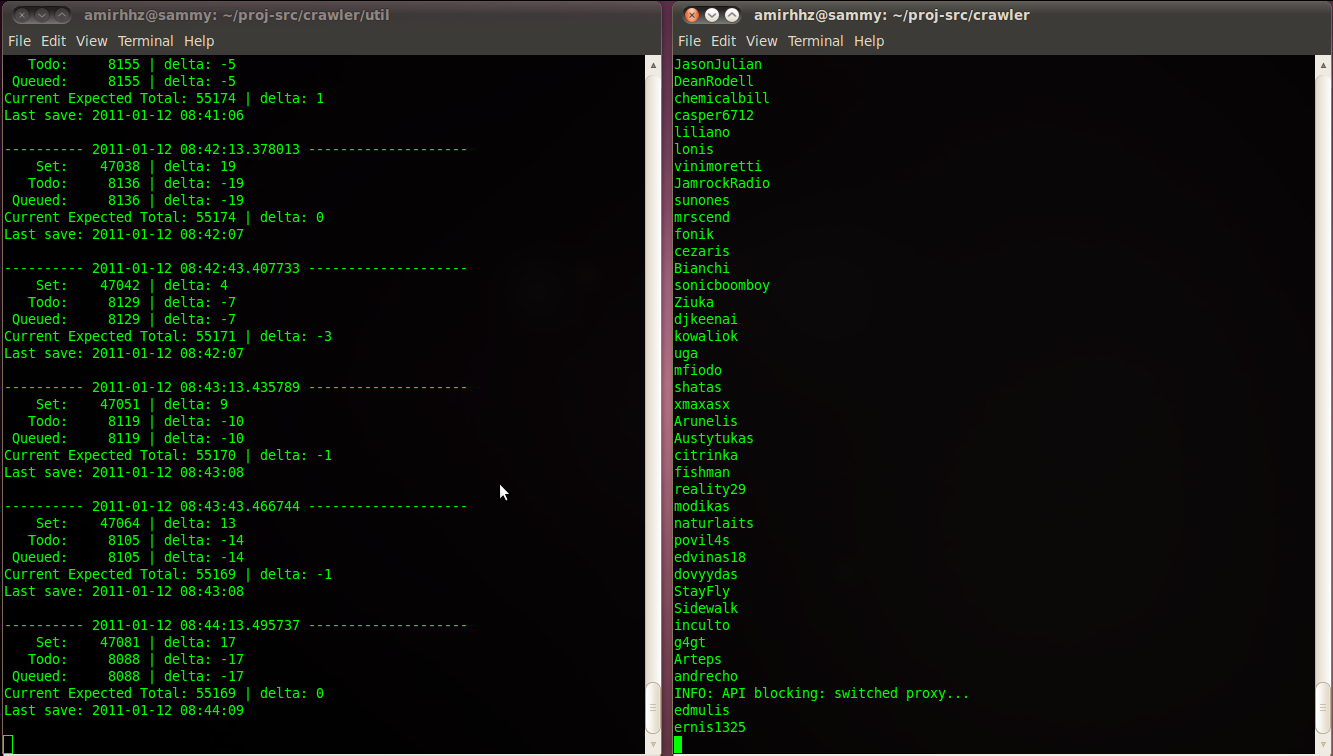
\includegraphics[width=\textwidth]{./images/running-scan.png}
 % running-scan.png: 1333x756 pixel, 72dpi, 47.03x26.67 cm, bb=0 0 1333 756
 \caption{The API Crawler running}
 \label{fig:running-scan}
\end{figure}

The crawler I wrote (see appendix \ref{app:crawler-code}) to download and store
the API data performed a breadth-first search of the graph once provided with a
few seed users and thus tried to get coverage of as much of the \mixurl\ social
graph as possible.

I decided to take a user-centric approach to the crawl, so in my database users
would be the first-class citizens and all other relevant data would be saved as
related to the users. In performing the graph search, I used all possible
features of a user to explore the graph: followers, followees, favourited items'
uploaders, and listened to items' uploaders.

\subsubsection{Redis: Semi-Persistent In-Memory Data Structures}

To keep track of my crawler's progress and graph search, I decided to use
Redis\footnote{\url{http://redis.io/}}. Redis is a key-value store, but with two
significant additions:
\begin{itemize}
 \item The values associated with each key can be high-performance lists, queues
and sets;
 \item The Redis server provides \emph{semi-persistence}, in that it
periodically and asynchronously writes the items in memory to disk, if enough
changes have been made, so the state of the data structures can be resumed later
or backed-up.
\end{itemize} 

Having these features in an existing tool meant that I did not have to implement
the respective functionalities from scratch in Python to aid my crawler. The
crawler would simply use Redis data structures to keep track of the queue of
users to remaining to download, and also use a set data structure that contained
the users who had already been downloaded to avoid fetching their data too
often upon multiple encounters.

\subsection{Storing the Data}

Thanks to MongoDB's excellent Python driver, storing the JSON responses of the
API were as simple as converting them to Python objects (see mapping table
\ref{tab:type-mapping}) and then calling the \texttt{save()} method on an
instance of a MongoDB collection.

I only faced a small problem at this stage. I was running MongoDB on 32-bit
operating systems and the designers of MongoDB have deliberately limited the
size of a database running on such OS's to 2GB per instance. Ideally I should
have been running a 64-bit OS. But I got around this issue by running several
instances of a MongoDB for each collection, instead of storing all collections
in one instance.

\section{Cleaning and Exploring the Data}

There were two sources of errors in the data I had gathered. Firstly, the
Mixcloud API had some bugs, specifically that sometimes the JSON fields that
showed the count of some feature of a user, for example
\texttt{favorite\_count}, did not match the actual number of favourites
associated with the user. Secondly, because my scan of the API would happen over
several days, there would be temporal inconsistencies (which I am calling
\emph{asymmetries}) in the data. By that I mean that references made in one
user's data would not have a corresponding reference in some other place because
that reference had been made during the time of the scan. For instance, someone
may have started following me on the second day of the scan, and because my user
data is collected on day one and the other person's data on day three, there
would asymmetric data in the dataset.

Cleaning the data to remove these errors was fairly straightforward. Correcting
the counts had to be performed first so that each user's data would be
consistent with itself before considering outside relationships. This was a
simple matter of running through each user and setting the count fields to
match the actual count of the features.

To solve the asymmetry problem, I decided to roll back the inconsistencies in
the graph until there no longer were any. I did this by identifying
inconsistencies first, and then removing excess references.

\subsection{Dataset Store Abstraction: MongoMix}

I wrote a library called \emph{MongoMix} that provided an abstraction layer
for the Mixcloud data I had stored in MongoDB and allowed me to access and
manipulate it programmatically in Python. The feature of MongoMix that helped
my later on was that I implemented a caching process for it to reduce the I/O
blocking penalty of accessing the data in the database from disk. By
pre-fetching data into the cache,I greatly improved the performance of
operations that worked on the entire dataset.


\section{Making Recommendations}

\subsection{Social Graph Model and Edge Prediction}

The dataset we have collected so far describes the social graph of \mixurl's
users. I am approaching the concept of recommendations as an edge prediction
problem for a graph, and the mechanism I have used to make the recommendations
for a given user is to find other users that are most similar to that user. The
candidate users for being recommended are those two hops away from the
recommendee in the social graph, because at more than two hops, almost the
entire graph would be covered. So the decisions that need to be made at this
stage are which similarity measures to use, and which features of the data to
base these measures on.

\subsection{Available Features}

The features that I can potentially use in calculating similarity measures for
users are:
\begin{itemize}
 \item followers,
 \item followees;
 \item favourited items' uploaders;
 \item listened-to items' uploaders.
\end{itemize}

These are the features that have social significance and whose association with
a user is likely provide signals as to who the user might have an affinity
towards and may want to form a social connection with.

\subsection{Similarity Measures}

The similarity measures I decided to use are as follows,
inspired by \cite{link-prediction}.

\begin{itemize}
 \item Intersection size: the amount of overlap between the features of two
users;
 \item Jaccard Co-efficient: intersection size divided by the size of the union
of the features, normalising the similarity value;
 \item Modified Jaccard: I modified the above measure to be the intersection
size over the smaller of the feature set, which means the normalisation is
relative to the maximum possible amount of overlap;
 \item Adamic-Adar\cite{adamic-adar}: Similar to the Jaccard Co-efficient but
refines the measure by weighting rarer features more heavily;
 \item Preferential Attachment: the size of two users' feature sets multiplied
together - this is normally a network-growth method, but it makes sense as a
similarity measure because one can think of the likelihood of two users being
connected as being proportional to how well-connected each of them are.
\end{itemize}


%%%%%%%%%%%%%%%%%%%%%%%%%%%%%%%%%%%%%%%%%%%%%%%%%%%%%%%%%%%%%%%%%%%%%%%%%%%%%%%
% Evaluation
\chapter{Evaluation}

The evaluation of my recommendations was based on making predictions on a test
dataset and comparing the results with a reference dataset to see if the
predictions occur.

\halfrule

\subsection{Producing Test Datasets}

For the snapshots of the dataset that I had gathered, I produced test versions
by removing some percentage (5-10\%) of all the edges in the network. Then I
could compare the recall and precision rates for the edge predictions that my
recommender produced.

Since I managed to capture three snapshots of the \mixurl\ dataset at 2 week
intervals, I could also use the organic growth of the data and treat each
snapshot as the test data for the next one.

For both types of test data, several parameters could be varied. The features
that would be used for the similarity calculations and the type of measure were
mentioned earlier. Also the threshold similarity value for including a
prediction as a recommendation could also be varied.

On the static snapshot with artificial edges removed, the performance of the
recommender was characterised by high rates (up to 50\%) of recall but at very
low precision, no more than 10\%. My modified Jaccard Co-efficient measure
seemed to perform best on these metrics.

Using the temporal snapshots to evaluate the recommender gave dismal results,
with both precision and recall rates being very close to zero.
%%%%%%%%%%%%%%%%%%%%%%%%%%%%%%%%%%%%%%%%%%%%%%%%%%%%%%%%%%%%%%%%%%%%%%%%%%%%%%%
% Conclusions
\chapter{Conclusions}

Making recommendations on evolving and dynamic data is difficult to do and
to measure. The nature of recommendations is that their real quality can only be
determined by the users whom they are presented to. I thought that using
temporal snapshots of data may be a good approximation to this, using the
actual behaviour of the users as groud truths for what recommendations should
be considered successful, but as demonstrated, this did not prove fruitful, at
least not with the approach I took.

I should also note that this project dissertation has fallen very short of
the expectations I had of it, and I want the reader to recognise my
disappointment with it. Much more sophisticated methods from the fields of
machine learning and information retrieval could have been explored, other
mature datasets used and obviously a much more thorough report could have been
written. Reasons as to why none of that happened are outside the scope of this
document, but I need to state that academia and I have unfinished business --
this isn't over.


%%%%%%%%%%%%%%%%%%%%%%%%%%%%%%%%%%%%%%%%%%%%%%%%%%%%%%%%%%%%%%%%%%%%%%%%%%%%%%%
% Bibliography

\addcontentsline{toc}{chapter}{Bibliography}
\bibliographystyle{abbrv}
\bibliography{refs}
\cleardoublepage

%%%%%%%%%%%%%%%%%%%%%%%%%%%%%%%%%%%%%%%%%%%%%%%%%%%%%%%%%%%%%%%%%%%%%%%%%%%%%%%
% Appendices

\lstset{numbers=left,numberstyle=\footnotesize\texttt}

\appendix
\chapter{Selected Source Code}

\section{Representation of the Connection to the API - api.py}
\label{app:api-code}

\lstinputlisting[language=Python,caption=Mixcloud API wrapper
source code, label=lst:api-code]{listings/api.py}

\clearpage

\section{API Crawler - crawler.api}
\label{app:crawler-code}

\lstinputlisting[language=Python,caption=The API data crawler
source code, label=lst:crawler-code]{listings/crawler.py}

\clearpage

\chapter{Original Project Proposal}

% to be included in proposal.tex

\author{Amir H. Hajizamani}
\title{CST Part II Individual Project Proposal -- Recommender Systems for Social Networks}


\newcommand{\al}{$<$}
\newcommand{\ar}{$>$}

\parindent 0pt
\parskip 6pt

\thispagestyle{empty}

\rightline{\large\emph{Amir H. Hajizamani}}
\medskip
\rightline{\large\emph{St. John's College}}
\medskip
\rightline{\large\emph{ahh29}}

\vfill

\centerline{\large Computer Science Tripos Part II Individual Project Proposal}
\vspace{0.4in}
\centerline{\Large\bf Recommender Systems for Social Networks}
\vspace{0.3in}
\centerline{\large{19 October 2010}}

\vfill

{\bf Project Originators:} Amir H. Hajizamani

\vspace{0.1in}

{\bf Resources Required:} See attached Project Resource Form

\vspace{0.5in}

{\bf Project Supervisor:} Cecilia Mascolo

\vspace{0.2in}

{\bf Signature:}

\vspace{0.5in}

{\bf Director of Studies:} Robert Mullins

\vspace{0.2in}

{\bf Signature:}

\vspace{0.5in}

{\bf Overseers:} Ann Copestake and Robert Harle

\vspace{0.2in}

{\bf Signatures:}

\vfill
\eject


\section{Introduction and Description of the Work}

In this project I will explore and implement techniques for making recommendations to members of online social networks. The motivation behind this idea is that the value of data about an individual person or some digital content (text, audio, video, etc.) is increased by knowledge of its relation to other such entities. This is true for the user, whose experience is enriched, and the service provider, whose cultural and financial success will depend on behaviour-based analysis and the growth and interactions of its users.

\subsection*{Motivation}

With the growing number of available social network services that individuals can choose to invest time and effort into, it is imperative that there is an incentive to do so. We take this investment by the user to consist of: providing personal information, creating and sharing content, making social connections with other users, and interacting with other users and content in the myriad of ways that are possible and observed in real world implementation such as Facebook, YouTube, LinkedIn, Twitter and Foursquare, to name a few. One way of providing this incentive is by making it easier for users to make \emph{discoveries} -- to find other individuals of interest (real-world friends, people with similar characteristics) or content. That is, make recommendations to users and keep them interested in exploring what the social network has to offer. Recommender systems aim to solve the problem of \emph{information overload} in areas where the users of a service struggle to make good choices on what content to consume or what social activities to take part in, simply because the options are overwhelming.

If we treat the users of a social network as a community, it is clear that the community will need the investment mentioned above from its users so that it reaches critical mass -- the point at which it is valuable for others to join or contribute to the network because the majority of their friends have, or so much of the content they consume is accessible via the service. This will continually increase the richness and quality of the service the community receives (assuming the service provider keeps up and adapts to changes!) and increase the lifetime and utility of the service for its users, too. Of course, here we are concerned with social networks that aim to reach the mainstream and are not inherently limited to a select number of users. For instance, a social network for the community of world experts on network congestion analysis is bound to hit its maximum membership limit very quickly and not be much more useful to its users than email or more traditional communication methods.

From a commercial perspective, which is arguably the more important one for the survival of a service, having users remain active on the network and incentivise others to do so, too, is paramount. It is well-understood that social network service providers are not expected to be profitable\footnote{\url{http://www.makeuseof.com/tag/how-do-social-networks-make-money-case-wondering/} -- explains the risks behind the business of social networks} until they reach an ``audience of scale'' to enable the adoption of a sensible monetisation model. For instance, Facebook only became profitable in 2009\footnote{\url{http://www.pcpro.co.uk/news/351646/facebook-eyes-profit-as-it-hits-300-million-members}} after reaching 300 million users. This means that the investors who enable such ventures at the start need to be convinced that the service has the potential to reach popularity and therefore provide a return on investment. Of the many strategies that can be used to maintain the growth of a social network, implementing a good recommender system is standard practice. It should be noted that recommendations are difficult, if not infeasible, to make at the very beginning of a network's lifetime due to the \emph{cold start} problem, that is, when there is insufficient data to base recommendations on. Therefore, the focus of this project is on stages of a network's lifetime after this issue has been overcome.

Below I describe my chosen dataset and the reasons for this choice over other available datasets.

\subsection*{The \emph{Mixcloud} Dataset}

I will work on data from Mixcloud.com whom I worked for over the summer of 2009. They are a steadily-growing and successful content distribution website, aiming to be the ``YouTube of Radio''. They provide a platform for user-generated audio content, ranging from podcasts to DJ mixes, to be easily accessed by anyone. They have been operating for over a year and have in the order of 100,000 users and a similar number of so-called ``Cloudcasts'' (uploaded audio content). They provide their users with social networking features such as Twitter-style following, Facebook-style activity updates, favouriting of Cloudcasts and commenting, and a record of listening history. The user-uploaded Cloudcasts are also heavily annotated with tags, categories, text descriptions, tracklists where appropriate, metadata about recent listeners and more. 

This wealth of metadata about their content and users is available via their public API\footnote{\url{http://api.mixcloud.com}} and I shall be gathering the data I need from it. The fact that the API is public means that I am able to use the data in my project and the results will be publishable in the project dissertation. I have had further confirmation from the staff at Mixcloud Ltd. about this.

At the time of writing, Mixcloud implement some simple mechanisms for \emph{item recommendations} and \emph{personalised recommendations} -- recommending Cloudcasts similar to the current one, and recommending Cloudcasts matching the user's personal listening history. I would like my recommender system to primarily aim to provide the functionality of \emph{social recommendations} -- suggesting other users whom the current user may be interested in following or listening to based on their shared social connections, activity similarities and other metrics. The problem of recommending content to users based on the listening pattern of their own social connections (as opposed to that of their entire community) can also be called \emph{social recommendation} and would likely use similar underlying data and metrics. I should point out that the social aspect of the Mixcloud community is more similar to that of Twitter, where people follow users who produce good content as well as real life friends, than that of Facebook where social links are more often initiated physically.

Following the motivations described earlier in the last subsection for recommender systems, I understand that Mixcloud have prioritised the implementation of Cloudcast recommendations on their website because their main focus has been on building up the library of content on their network and promoting themselves as content distributors. However, the social networking layer on top of their distribution layer is naturally their next focus, whilst they improve the recommendation algorithms they currently use, too. They can leverage the high standard of their content metadata and existing social connections to make social recommendations. So essentially, the quality and completeness of the dataset, despite its organic nature, and the utility of a social recommender system for Mixcloud and their community are good reasons for picking it. I also compare the Mixcloud dataset with other ones traditionally used to explore recommender system techniques below.

A working system would likely draw on concepts from all three types of recommendation mentioned so far to account for inherent peculiarities in the dataset. For example, two users may have common taste in music but not be well-connected in the social graph or vice-versa. An effective system would take advantage of the rich social graph and indirect relationships between users and content to overcome these issues and enable further linkage in the dataset, hopefully with the effect of aiding the community and commercial objectives outlined so far.

\subsubsection*{Comparison with other Available Datasets}

The most widely used datasets in discussions on recommender systems are the MovieLens, EachMovie, Book-Crossing and Jester Jokes datasets\footnote{\url{http://www.grouplens.org/node/12} -- all of these datasets are available via this link} which contains items and user ratings on their respective titular item types. Though the quality of these datasets is proven, they have limitations for my intended project goals. In particular, there is no social connectivity data between users in these datasets and the links between entities are limited to ratings by users on some items. With the Mixcloud dataset I am able to explore the social graph of the users. Furthermore, the Mixcloud dataset provides much richer metadata about its entities, as described above, than any of the traditional datasets which give only enough data to build item-item and item-user matrices corresponding the ratings. The Mixcloud dataset has scope for more interesting analysis and recommender system implementations.

The Mixcloud dataset also has the potential for analysis in the temporal dimension, which is the extension idea for this project and is described later in this document.

\subsection*{Wider Context}

The Web is rife with successful recommender systems, with companies such as \textit{Amazon, Netflix\footnote{In 2006 Netflix challenged programmers to improve their movie recommendation engine by 10\%.}} and \textit{Pandora} (radio service backed by \textit{The Music Genome Project}\footnote{\url{http://www.pandora.com} -- The MGP uses the``genealogy'' of music to link songs and artists}) investing a lot of time and money in improving their algorithms and data quality to better recommend items of interest to their users. On the other hand, more directly community-driven websites such as \textit{del.icio.us} and \textit{flickr} have harnessed the collective intelligence of their users and their tagging of their content with keywords. Collaborative tagging leads to an organic categorisation and annotation of data which has been termed \textit{folksonomy}\footnote{\url{http://www.vanderwal.net/folksonomy.html} -- a portmanteau of \textit{folk} and \textit{taxonomy} }. In a sufficiently large and active community, the folksonomy that can be extracted becomes a good source of input for the algorithms in a recommender system. 

With the accelerating growth of social networks such as Twitter and Facebook, the value of social recommendations which aim to increase the connections between individuals is more important that it used to be: the items of interests are now other users not products on sale (though from an advertising revenue perspective the difference is blurred). Recommender systems are nearing maturity and will soon be, if they are not already, commodity technologies as the ``social connections layer'' of virtual communities is completed\footnote{The ``game layer'' is the next stage in building virtual communities, the founder of SCVNGR argues -- \url{http://www.ted.com/talks/seth_priebatsch_the_game_layer_on_top_of_the_world.html}}. This means that an analysis of such systems is essential to the understanding of social networking and the Web as it experiences a paradigm shift from a \emph{search} platform (e.g. Google) to a \emph{discovery} platform.

\section{Starting Point}

I am familiar with the RESTful\footnote{Representational State Transfer-style access to data over HTTP/1.1. This particular API responds to requests in the JSON data interchange format.} API provided by Mixcloud which I have already begun obtaining data from. At the time of writing, I have collected data on approximately 20000 users by performing a breadth-first search on the social connections of a few hand-picked seed users. 

What I have learned from some of the Computer Science Tripos courses such as Artificial Intelligence I, Digital Communications I and Databases will likely help me along the way.

The type of algorithms I will be using in this project will be new to me and my only exposure to them is in reading the relevant literature.
  
\section{Substance and Structure of the Project}

The data for the project will be obtained over the Mixcloud API as JSON objects and stored in the documented-oriented database, MongoDB. This will involve writing a crawler application to explore the social and content graph of Mixcloud via its API and save the relevant result in a useful way. As mentioned above, I have already begun doing this, writing a wrapper for the API in Python to use in my crawler application.

As I mentioned in the above section, I have no prior experience of the types of processing and algorithms used in building recommender systems and therefore I will have to spend some time examining the existing literature and open source code.

Building a recommender system involves the following broad stages: 
\begin{itemize}
 \item Identifying appropriate distance metrics to measure the similarity or relevance of item-item, item-user and user-user pairs;
 \item Computing the above metrics for the available data;
 \item Make recommendations with appropriate classification and filtering alogirthms, using these metrics.
\end{itemize}

\subsection*{Data for Distance Metrics}


A common notion in recommender system design is that of ``ratings'' for a particular entity on some scale. Within the Mixcloud dataset, ratings are uniformly binary, that is, the existance of a connection between two entities signifies an implicit or explicit preference rating, and the lack of a connection means no implicit or explicit rating is available. These so-called ratings between entities can be used to measure the similarity or relevance, which I shall collectively call distance, of entities in the social network. The techniques used to measure distance between two entities of the same type can be similar whether the entities are Cloudcasts (items) or users. These can then be used to calculate the mixed-type distances, that is, the relevance of a Cloudcast to the active user and vice-versa.

A distance metric for measuring item-item distance could use the following ratings and objects as it's input data: 
\begin{itemize}
 \item The sets of users who have listened to/favourited/commented on/uploaded the two items in question
 \item The sets of tags and other metadata carried by the two items 
\end{itemize}


Similarly, a metric for measuring social relevance -- whether a user-user pairing should exist between two individuals -- can use the following:
\begin{itemize}
 \item Association: the two users' sets of current social links -- followers, followees, profile commentors. 
 \item Taste and Activity: the two users' sets of listening history/favourites/Cloudcast comments.
 \item In-Depth Taste: the metadata carried by the users' uploads/favourites/listening history.
\end{itemize}

The actual distance metrics that I will use will be subject to other implementation details. 

\subsection*{Classification and Filtering}

The fundamental process that my proposed recommender system will perform is to classify a relationship between two entities as either existing or not existing, taking into account the distance metrics discussed above. Given two users, two Cloudcasts, or a user and a Cloudcast, should a recommendation be made for linking them? The decision to be made is a binary one and the family of machine learning techniques used for this kind of processing are \emph{binary classifiers}. These are a class of algorithms which employ probabilistic models derived from some training data to make prediction about further unseen data.

Reading the relevant literature, the classic approach to making recommendations is to use \emph{Collaborative Filtering} (CF) techniques, which aim to make predictions for a given user or item based on data available for similar users or items. CF techniques can be split into two main types: memory-based and model-based. I am more interested in the model-based solutions to CF because I wish to build a recommender system that identifies complex patterns in data using machine learning techniques, as mentioned above. The memory-based approach is simple to implement but limited -- essentially large sparse matrices of entity relationships/distances are stored and for a given entity the highest ranking corresponding entities are given as recommendation. This naturally has the problem that for changes in the set of entities recomputation of the matrices is required and also with large data sparsity, the computational performance of the system suffers.

\section{Success Criterion}

The main method of evaluation I will use to judge the success of the recommender system I write will be cross-validation of the system performance over samples of the dataset. This is a common technique for assessing the performance of a supervised learning system which aims to make predictions on some test data, given some training data. This process would involve splitting the dataset into some number $n$ of disjoint partitions and for each partition removing some of the links between entities (nodes in the network). The system is then optimised for making recommendations that repair the broken links in some $k, (k < n)$ subset of these partitions (the training data) and comparing its performance on the remaining $(n-k)$ partitions (the test data). Some of the metrics that can be used to measure the performance of the system are the precision (the proportion of the results that are correct ones) and recall (the proportion of the correct items that appear in the result) rates\cite{eval_measures} in the context of classifier performance evaluation. 

\section{Extension Ideas}

\subsection*{The Temporal Dimension}
If I am able to obtain several snapshot of the social network across time, perhaps at 3-4 week intervals, I could use the snapshots as a means of evaluation by comparing recommendations made for the network at time (snapshot) $t-1$ with the changes made to the network at time $t$. This method of evaluation of the recommender system will compare the performance of the recommender system against the organic growth and changes in the real network since a previous snapshot.


\section{Resources Required}
See attached Project Resource Form. I have included a summary below:
\begin{itemize}
\item Mixcloud.com user and content data from their API -- a cautious estimated size of 2GB
\item PWF Filespace -- Up to 500Mbytes
\item SRCF Filespace  -- Up to 500Mbytes
\item My own Laptop PC (Intel Core 2 Duo T6400 2.0GHz, 4GB RAM, 500GB HHD)
\end{itemize}

\section{Timetable and Milestones}

From the official beginning of this project on Fri 23rd October until the submission deadline of Fri 20th May, there are 30 weeks which I have timetabled as follows:

\textbf{22 Oct -- Submission of this Proposal}

\textbf{23 Oct -- 5 Nov}

Have a usable sample of the dataset gathered from the Mixcloud API and be comfortable with manipulating the database programmatically.
Ensure backup strategies and project management practices are in place.

\textbf{6 Nov -- 26 Nov}

Implement the basic methods for calculating distance metrics.
Ensure I have an understanding of the mathematical properties of the metrics and their suitability for my application.

\textbf{27 Nov -- 10 Dec}

Implement some classifiers and Collaborative Filtering algorithms with appropriate distance metrics - these should produce meaningful output given some small simple input.
At the end of this time, I should be comfortable with the various data structures, algorithms and techniques available to me to implement a recommender system.
I also need to ensure that I understand all the evaluation methods available for these techniques.

\textbf{11 Dec -- 7 Jan}

Using knowledge gained so far, build a recommender system that produces meaningful results given a large, realistic input, combining and experimenting with different techniques as discussed above.

\textbf{8 Jan -- 21 Jan}

Start planning out the dissertation, with the Introduction and Preparation chapters being nearly complete and the Implementation chapter beginning to take form.

\textbf{22 Jan -- 3 Feb}

Prepare for the progress report by testing the working recommender system and doing preliminary evaluation on it. Producing some visualisations and graphics from the data and the output will also be helpful for this, as well as for the final dissertation. 
Produce the presentation for progress report.

\textbf{4 Feb -- Submission of Progress Report}

\textbf{5 Feb -- 18 Feb}

Work on any feedback from progress report.
Begin work on more advanced techniques or novel approaches that I may have come up with after using the data, e.g. Temporal Analysis.
Set out a clear plan for evaluating the performance of the recommender, including the type of measurements to be taken and comparisons to draw.

\textbf{19 Feb -- 4 Mar}

Analyse performance of the system and move onto extensions in earnest.
Final clean up of code and extensions.
Dissertation document is regularly updated during this time and the Implementation section has taken form.

\textbf{5 Mar -- 25 Mar}

Dissertation is comfortably on target in terms of content and word limit.
Identify weaknesses in code and documentation, and address them.

\textbf{26 Mar -- 13 May}

Final proof reading of dissertation and aim to submit a week before deadline.

\textbf{20 May -- Submission of Dissertation}

\begin{thebibliography}{}
 \bibitem{eval_measures} R. Eisner, Basic Evaluation Measures for Classifier Performance -- \url{http://www.cs.ualberta.ca/~eisner/measures.html} -- this page describes the terms \textit{recall, precision, accuracy and specificity}.
 \bibitem{eval_cfsys} J. L. Herlocker et al., Evaluating Collaborative Filtering Recommender Systems, ACM Transactions on Information Systems, Vol. 22, No. 1, January 2004
 \bibitem{survey_cf} X. Su et al, A Survey of Collaborative Filtering Techniques, Advances in Artificial Intelligence, Volume 2009
 \bibitem{analysis_recsys_algs} E. Vozalis et al., Analysis of Recommender Systems’ Algorithms


\end{thebibliography}

\cleardoublepage

\end{document}
